\documentclass[12pt,a4paper]{report}

\setlength{\topmargin}{0 cm}
\usepackage{times}
\usepackage{float}
\usepackage{rotating}
\usepackage[german]{babel}
\usepackage{graphics}
\graphicspath{ {../img/} {../graph/img/} }
\usepackage{color}
\usepackage{caption}
\usepackage{subcaption}
\usepackage{ntheorem}
\theoremstyle{break}
\theorembodyfont{\normalfont}
\theoremprework{\bigskip\hrule\leavevmode\nopagebreak}
\theorempostwork{\nopagebreak\hrule\leavevmode}
\newtheorem{exercise}{Aufgabe}[chapter]
\theoremstyle{plain}
\theoremprework{\bigskip\hrule\leavevmode\nopagebreak}
\theorempostwork{\nopagebreak\hrule\leavevmode}
\newtheorem{proof}{Satz}[chapter]
\renewcommand{\labelenumii}{\arabic{enumi}.\arabic{enumii}.}
\newcommand{\algostep}[2]{\parbox{4cm}{\scalebox{0.5}{\includegraphics{#1}}}
  \hfill
  \parbox{7cm}{#2}
}
\title{Minimale Spannb\"{a}ume}
\author{Gabriel Katz\\ Matthias Neeracher}

\begin{document}
\maketitle
\tableofcontents
\chapter{Einleitung}

\section{Worum geht es hier?}

In den fr\"uhen 20er Jahren besch\"aftigte sich der 
Mathematiker Otakar Bor\r{u}vka mit dem Problem, ein Gebiet (40
St\"{a}dte in S\"{u}d-M\"{a}hren) m\"{o}glichst effizient mit 
Elektrizit\"{a}t zu erschliessen.

\begin{figure}[h!]
\resizebox{!}{4cm}{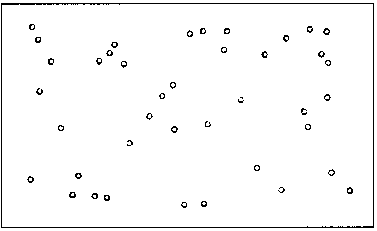
\includegraphics{BoruvkaPoints.pdf}}
\resizebox{!}{4cm}{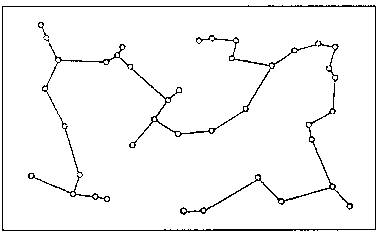
\includegraphics{BoruvkaTree.pdf}}
\caption{Elektrische Erschliessung von S\"{u}d-M\"{a}hren.\protect\footnotemark}
\end{figure}

\footnotetext{ 
Otakar  Bor\r{u}vka, \emph{O jist\'{e}m probl\'{e}mu minim\'{a}ln\'{i}m} (\"{U}ber ein
  gewisses Minimalisierungsproblem). \\
Zitiert aus: J. Ne\v{s}et\v{r}il,
  E. Milkov\'{a}, H. Ne\v{s}et\v{r}ilov\'{a}, \emph{Otakar Bor\r{u}vka
    on minimum spanning tree problem: translation of both the 1926
    papers, comments, history.}, Discrete Mathematics 233 (2001)}
Sein Ansatz war, das Problem als \textbf{Graphen} abzubilden, in dem die
anzuschliessenden St\"{a}dte als \textbf{Knoten}, und die Distanzen zwischen ihnen
als \textbf{Kanten} repr\"{a}sentiert wurden. Das Elektrifizierungsproblem
besteht somit darin, alle Knoten so zu verbinden, dass die
Gesamtl\"{a}nge der Kanten so kurz wie m\"{o}glich bleibt. Eine solche
Verbindung wird \textbf{minimal aufspannender Baum} oder kurz
\textbf{minimaler Spannbaum} genannt.

Bor\r{u}vka's L\"{o}sung, die er 1926 publizierte, gilt als der erste
Algorithmus zur Konstruktion eines minimalen Spannbaums, und als einer
der ersten Optimierungs-Algorithmen. Weil sowohl
die Problemstellung als auch die verwendeten Algorithmen interessant
und einigermassen leicht verst\"{a}ndlich sind, werden wir uns jetzt diesem Problem widmen.
\section{Wie kann hier gearbeitet werden?}

Dieser Text wird Sie mit einem wichtigen algorithmischen Problem
bekannt machen: dem Finden eines minimalen Spannbaums. Im n\"{a}chsten
Abschnitt finden Sie eine Einf\"{u}hrung in das Thema, doch bevor
Sie loslegen, soll Ihnen hier noch kurz der Aufbau des Textes und die
Arbeitsweise damit erl\"{a}utert werden.

Die folgenden Kapitel sind zur selbstst\"{a}ndigen Bearbeitung
gedacht. Sie werden zuerst kurz Ihre Kenntnisse von ungerichteten
Graphen nochmals auffrischen, lernen dann die Theorie von B\"{a}umen
und gewichteten Graphen kennen, und lernen dann zwei verschiedene
Algorithmen, um einen \emph{minimalen Spannbaum} zu finden.
 
Wenn Sie einige dieser Begriffe jetzt noch nicht verstehen, macht das
nichts. Mitbringen sollten Sie aber die folgenden Kenntnisse:

\begin{itemize}
\item Sie wissen, was ein Algorithmus ist.
\item Sie kennen die Grundbegriffe ungerichteter Graphen (wir werden
  diese allerdings in Kapitel~\ref{graphs} kurz repetieren).
\end{itemize}

Zur behandelten Theorie finden Sie immer auch Aufgaben, anhand derer
Sie das Gelernte pr\"{u}fen k\"{o}nnen. Die L\"{o}sungen dieser Aufgaben stehen
jeweils im zweitletzten Unterkapitel f\"{u}r jedes Thema. Das letzte
Unterkapitel ist dann der Kapiteltest, den Sie bearbeiten und mit
Ihrer Lehrperson besprechen sollten.

\newpage
\chapter{Graphen}
\label{graphs}
In diesem Kapitel frischen wir unsere Kenntnisse zur Graphentheorie
auf. Zuerst repetieren wir, was ein Graph \"{u}berhaupt ist und wie er
dargestellt werden kann. Danach betrachten wir zwei Konzepte,
n\"{a}mlich zusammenh\"{a}ngende Graphen und Teilgraphen, welche
f\"{u}r die n\"{a}chsten Kapitel wichtig sind. Am Ende des Kapitels
behandeln wir noch die gewichteten Graphen. Wenn Sie sich bereits
in all diesen Themen sattelfest f\"{u}hlen, k\"{o}nnen Sie direkt den
Kapiteltest in Abschnitt~\ref{graphchaptest} in Angriff nehmen.

\section{Rekapitulation: Was ist ein Graph?}

Ein \textbf{Graph} $G(V,E)$ besteht aus einer Menge von
\textbf{Knoten} $V$ und einer Menge von Kante $E$. Eine \textbf{Kante}
besteht aus einem Paar von Knoten, den \textbf{Endknoten} der
Kante. Wenn diese Paare geordnet sind, ist der Graph
\textbf{gerichtet}; die Kanten verbinden die Knoten nur in eine
Richtung. 

In diesem Text befassen wir uns aber nur mit
\textbf{ungerichteten} Graphen, in welchen die Knotenpaare ungeordnet
und somit die Knoten symmetrisch verbunden sind.  Des weiteren
beschr\"{a}nken wir uns auf \textbf{einfache} Graphen, in denen keine
Kanten einen Knoten mit sich selbst verbinden, und zwischen zwei
Knoten nicht mehr als eine Kante existiert.

\begin{exercise}\label{exgerichtet}
Welche dieser vier Graphen sind gerichtet, welche ungerichtet? Welche
sind einfach?
\begin{figure}[H]
\begin{subfigure}[b]{0.23\textwidth}
\scalebox{0.4}{\includegraphics{UngerichtetUnschlicht.pdf}}
\caption{}
\end{subfigure}
\begin{subfigure}[b]{0.23\textwidth}
\scalebox{0.4}{\includegraphics{Gerichtet.pdf}}
\caption{}
\end{subfigure}
\begin{subfigure}[b]{0.23\textwidth}
\scalebox{0.4}{\includegraphics{Ungerichtet.pdf}}
\caption{}
\end{subfigure}
\begin{subfigure}[b]{0.23\textwidth}
\scalebox{0.4}{\includegraphics{GerichtetUnschlicht.pdf}}
\caption{}
\end{subfigure}
\caption{Welche der Graphen sind gerichtet? Welche einfach?}
\end{figure}
\end{exercise}

\section{Beschreibung von Graphen}
\label{Beschreibung}
\noindent Ein Graph $G(V,E)$ kann auf verschiedene Arten beschrieben werden:

\begin{description}
\item[Grafisch] indem die Knoten und Kanten aufgezeichnet werden:

\begin{figure}[H]
\centerline{
\scalebox{0.5}{\includegraphics{Ungerichtet.pdf}}
}
\caption{Grafische Darstellung eines Graphen}
\label{fig:GrafischeDarstellung}
\end{figure}
gerade bei kleineren Graphen ist diese Darstellung f\"{u}r Menschen am
Einfachsten zu verstehen, aber sie ist z.B. f\"{u}r
Computerverarbeitung nicht besonders gut geeignet.
\item[Mengentheoretisch] indem die Knoten- und die Kantenmenge
  beschrieben werden:

\begin{displaymath}
V = \{\mathsf{A,B,C,D,E}\}\hspace{2cm}E = \{\mathsf{\{A,B\}, \{B,C\},
  \{C,D\}, \{C,E\}, \{B,E\}}\}
\end{displaymath}

\item[\textnormal{als} Adjazenzmatrix] indem die Kanten als $n\times{n}$ Matrix $A(G)$
  dargestellt werden, wo der Eintrag $a_{ij}$ gleich $1$ ist, wenn eine Kante
  von Knoten $i$ nach Knoten $j$ existiert, und sonst gleich $0$.

\begin{displaymath}
A(G) = \left( 
\begin{array}{ccccc}
0 & 1 & 0 & 0 & 0 \\
1 & 0 & 1 & 0 & 1 \\
0 & 1 & 0 & 1 & 1 \\
0 & 0 & 1 & 0 & 0 \\
0 & 1 & 1 & 0 & 0 
\end{array}
\right)
\end{displaymath}

Wie zu beobachten ist, ist die Adjazenzmatrix bei einem ungerichteten
Graphen immer symmetrisch.
\end{description}

\begin{exercise}\label{exrep}
\begin{itemize}
\item Zeichnen Sie einen ungerichteten Graphen $G(V,E)$ mit Knoten 
$V = \{\mathsf{A,B,C,D,E}\}$ und Kanten 
$E = \{\mathsf{\{A, B\}, \{A, D\}, \{C, D\}, \{A, E\}}\}$.
\item Konstruieren Sie die Adjazenzmatrix dieses Graphen.
\end{itemize}
\end{exercise}

\section{Zusammenh\"{a}ngende Graphen}

Wenn in einem Graphen $G(V,E)$ eine Folge von Knoten $(v_0, v_1,
\ldots, v_n)$, $v_i \in V$ existiert, die von Kanten $e_i = \{v_i, v_{i+1}\} \in
E$ verbunden werden, dann existiert ein \textbf{Weg} von $v_0$ nach
$v_n$. 

Falls ein Weg f\"{u}r \emph{jedes} Knotenpaar $v_0, v_n
\in V$ existiert, nennen wir den Graphen \textbf{zusammenh\"{a}ngend}.

Ob ein Graph zusammenh\"{a}ngend ist, l\"{a}sst sich intuitiv recht
einfach in seiner grafischen Darstellung verstehen: Ein Graph
ist zusammenh\"{a}ngend, wenn alle Knoten miteinander verbunden sind. Sind
die Knoten nicht alle miteinander verbunden, so heissen die verbundenen Teile des 
Graphen \textbf{Komponenten}.

Ein Weg $v_0,v_1,\ldots,v_n,{v_0}$, der von einem Knoten
$v_0$ wieder auf diesen selbst zur\"{u}ckf\"{u}hrt, heisst
\textbf{geschlossen}.

\begin{exercise}\label{exverbund}
Welcher der folgenden Graphen ist zusammenh\"{a}ngend? Markiere bei den nicht zusammenh\"{a}ngenden Graphen die
gr\"{o}sste Komponente.

\begin{figure}[H]
\begin{subfigure}[b]{0.3\textwidth}
\scalebox{0.4}{\includegraphics{ConnectedComponents1.pdf}}
\caption{}
\end{subfigure}
\begin{subfigure}[b]{0.3\textwidth}
\scalebox{0.4}{\includegraphics{ConnectedComponents2.pdf}}
\caption{}
\end{subfigure}
\begin{subfigure}[b]{0.3\textwidth}
\scalebox{0.4}{\includegraphics{ConnectedComponents3.pdf}}
\caption{}
\end{subfigure}

\caption{Welcher Graph ist zusammenh\"{a}ngend?}
\end{figure}

\end{exercise}

\newpage
\section{Teilgraphen}

Ein Graph $U(W,F)$ ist ein \textbf{Teilgraph} eines Graphen $G(V,E)$
wenn seine Knotenmenge $W$ eine Teilmenge der Knotenmenge $V$ ist und
seine Kantenmenge $F$ eine Teilmenge der Kantenmenge $E$.
Ein Teilgraph $U(W,F)$ eines Graphen $G$ ist \textbf{aufspannend}, 
wenn $W=V$. Ein aufspannender Teilgraph muss weder zusammenh\"{a}ngend sein, noch muss jeder Knoten mit einer Kante verbunden sein.
\begin{exercise}\label{exunter}
Welche der folgenden drei Graphen sind Teilgraphen des Graphen aus
Abbildung~\ref{fig:GrafischeDarstellung}?

\begin{figure}[H]
\begin{subfigure}[b]{0.3\textwidth}
\scalebox{0.4}{\includegraphics{Sub1.pdf}}
\caption{}
\end{subfigure}
\begin{subfigure}[b]{0.3\textwidth}
\scalebox{0.4}{\includegraphics{Sub2.pdf}}
\caption{}
\end{subfigure}
\begin{subfigure}[b]{0.3\textwidth}
\scalebox{0.4}{\includegraphics{Sub3.pdf}}
\caption{}
\end{subfigure}

\caption{Welche Graphen sind Teilgraphen?}
\end{figure}

\end{exercise}
\begin{exercise}\label{excompletesubgraph}
Ein \emph{vollst\"{a}ndiger} Graph $K_n$ ist ein Graph mit $n$ Knoten, in welchem jedes Knotenpaar mit einer Kante verbunden ist.
\[ 
K_n(V = \{v_1, v_2, \ldots, v_n\}, E = \{\{v_a, v_b\} \mid v_a, v_b \in V,
v_a \neq v_b\})
\] 
\begin{itemize}
\item Finde eine Formel f�r die Anzahl Kanten in $K_n$
\item \textbf{(FAKULTATIV)} Wie viele aufspannende Teilgraphen hat $K_2$? Wieviele $K_3$? Finde eine Formel, um die Anzahl Kanten von $K_n$ zu berechnen.
\end{itemize}
\end{exercise}

\newpage
\section{Gewichtete Graphen}
\label{gewichtet}

In vielen praktischen Anwendungen sind die Knoten und/oder Kanten
eines Graphen mit \textbf{Gewichten} versehen. Die Kantengewichte k\"{o}nnen
z.B. Distanzen oder Flugkosten darstellen, die Knotengewichte
z.B. Hotelkosten.

\begin{exercise}\label{extravel}
Der folgende Graph zeigt Flug- und Hotelkosten, sowie Reisedistanzen
f\"{u}r eine Reise. Wir nehmen an, dass der Reisende bei jedem Zwischenhalt eine Nacht in einem Hotel \"{u}bernachten muss.
Bei Start- und Endpunkt der Reise, also, Z�rich und Sidney, ist keine \"{U}bernachtung n\"{o}tig. Daher sind im Graph auch 
keine Kosten aufgef\"{u}hrt.
\begin{figure}[H]
\centerline{
\scalebox{0.5}{\includegraphics{Travel.pdf}}
}
\caption{Flug- und Hotelkosten und Reisedistanzen}
\end{figure}
\begin{enumerate}
\item Was ist die \emph{k\"{u}rzeste} Route zwischen Z\"{u}rich und
    Sydney?
\item Was ist die \emph{billigste} Route, wenn man die Hotelkosten bei jeder Zwischenlandung ber�cksichtigt?
\end{enumerate}
\end{exercise}

In der weiteren Diskussion werden wir hier nur noch an \textbf{Kantengewichteten} Graphen interessiert sein.

\newpage
\section{L\"{o}sungen}

\begin{description}
\item[Aufgabe~\ref{exgerichtet}] \hfill \\[0cm]
\begin{enumerate}
\item Ungerichtet, nicht schlicht weil $C$
  mit sich selbst verbunden ist. 
\item Gerichtet und schlicht. 
\item Ungerichtet
  und schlicht. 
\item Gerichtet, nicht schlicht weil zwischen $B$ und $E$
  zwei Kanten existieren.
\end{enumerate}
\item[Aufgabe~\ref{exrep}] \hfill \\[0cm]
\algostep{Exrep.pdf}{
\begin{displaymath}
\left( 
\begin{array}{ccccc}
0 & 1 & 0 & 1 & 1 \\
1 & 0 & 0 & 0 & 0 \\
0 & 0 & 0 & 1 & 0 \\
1 & 0 & 1 & 0 & 0 \\
1 & 0 & 0 & 0 & 0 
\end{array}
\right)
\end{displaymath}}
\item[Aufgabe~\ref{exverbund}] Graph (a) ist nicht verbunden. Die 
gr\"{o}sste Komponente besteht aus den  Knoten $A$, $B$ und $C$.
Graph (b) ist zusammenh\"{a}ngend. Graph (c) ist nicht zusammenh\"{a}ngend. Die 
gr\"{�}sste Komponente besteht aus den  Knoten $A$, $B$, $C$ und $E$.
\item[Aufgabe~\ref{exunter}] Graphen (a) und (c) sind Teilgraphen (Ein Teilgraph muss
  \emph{nicht} notwendig zusammenh\"{a}ngend sein). Graph (b)
  enth\"{a}lt eine Kante $\{A,C\}$ die im urspr\"{u}nglichen Graphen
  nicht existiert. 
\item[Aufgabe~\ref{excompletesubgraph}] 
Ein kompletter Graph $K_n$ hat $n(n-1)/2$ Kanten. F\"{u}r jede Kante 
wird die Anzahl der m\"{o}glichen Teilgraphen verdoppelt, da die Kante 
entweder im Teilgraphen vorkommen kann oder nicht. Somit hat $K_2$ zwei
verschiedene Teilgraphen, $K_3$ hat acht Teilgraphen, und $K_n$ hat $2^{n(n-1)/2}$ spannende
Teilgraphen.
\item[Aufgabe~\ref{extravel}]\hfill\linebreak
\begin{enumerate}
\item Z\"{u}rich---Singapur---Sydney (16589 km)
\item Z\"{u}rich---Moskau---Ulan Bator---Sydney (Fr. 3400.-)
\end{enumerate}
\end{description}

\section{Kapiteltest}\label{graphchaptest}

\begin{exercise}\label{test1adjacency}
Gegeben sei die Adjazenzmatrix f\"{u}r einen Graphen $G$.

\begin{displaymath}
A(G) = \left(
\begin{array}{ccccccc}
0 & 1 & 0 & 0 & 0 & 0 & 0 \\
1 & 0 & 0 & 1 & 0 & 0 & 0 \\
0 & 0 & 0 & 0 & 0 & 0 & 0 \\
0 & 1 & 0 & 0 & 1 & 0 & 0 \\
0 & 0 & 0 & 1 & 0 & 0 & 0 \\
0 & 0 & 0 & 0 & 0 & 0 & 1 \\
0 & 0 & 0 & 0 & 0 & 1 & 0 
\end{array}
\right)
\end{displaymath}

\begin{enumerate}
\item Zeichnen Sie den Graphen auf (verwenden Sie $A..G$ als
  Knotennamen).
\item Stellen Sie den Graphen in Mengennotation dar.
\item Aus welchen Komponenten besteht der Graph?
\end{enumerate}

\end{exercise}

\begin{exercise}\label{test1weights}
Gegeben sei der folgende Graph:

\scalebox{0.5}{\includegraphics{SubWegGewicht.pdf}}

\begin{enumerate}
\item Welcher Weg von $A$ nach $D$ weist die kleinste Summe von
  Kantengewichten auf?
\item Welcher geschlossene nichtleere Weg im Graphen weist die kleinste Summe von
  Kantengewichten auf?
\end{enumerate}

\end{exercise}

\section{L\"{o}sung zum Kapiteltest}
\begin{description}
\item[Aufgabe~\ref{test1adjacency}] \hfill \\[0cm]
\begin{enumerate}
\item 
\begin{figure}[H]
\centerline{
\scalebox{0.5}{\includegraphics{kapiteltest1.pdf}}
}
\end{figure}

\item $G = (V,E)$, $V = \{A, B, C, D, E\}$, $E=\{ \{A, B\}, \{B, D\},\{D, E\},\{F, G\}\}$.
\item Der Graph besteht aus drei Komponenten. Die Knoten $A$,$B$,$D$ und $E$ und die Kanten dazwischen bildet 
eine Komponente, Knoten $C$ ist die zweite Komponente, und $F$ und $G$ mit der Kante dazwischen bildet die dritte Komponente.
\end{enumerate}

\item[Aufgabe~\ref{test1weights}] \hfill \\[0cm]
\begin{enumerate}
\item $A, E, C, D$ hat eine Kantengewichtsumme von nur $7$.
\item $A, B, C, E, A$ hat eine Kantengewichtsumme von $13$.
\end{enumerate}
\end{description}

\chapter{B\"{a}ume}

\section{Was ist ein Baum?}

Als \textbf{Baum} bezeichnen wir einen Graphen, der
\emph{zusammenh\"{a}ngend} ist und \emph{keinen geschlossenen Weg}
enth\"{a}lt. Eine Menge von B\"{a}umen, die keine gemeinsamen Knoten
haben, bezeichnet man (anschaulicherweise) als \textbf{Wald}.

\begin{figure}[h!]
\begin{subfigure}[b]{0.35\textwidth}
\resizebox{!}{5cm}{\includegraphics{BaumBsp.pdf}}
\caption{}
\end{subfigure}
\begin{subfigure}[b]{0.6\textwidth}
\resizebox{!}{7cm}{\includegraphics{WaldBsp.pdf}}
\caption{}
\end{subfigure}
\caption{Ein Baum (a) und ein Wald (b)}
\end{figure}

\begin{exercise}\label{exbaum}
Welche der folgenden drei Graphen sind B\"{a}ume? Gestalten Sie die
anderen Graphen durch Hinzuf\"{u}gen bzw. Weglassen von geeigneten
Kanten so um, dass sie ebenfalls zu B\"{a}umen werden.

\begin{figure}[h!]
\begin{subfigure}[b]{0.3\textwidth}
\scalebox{0.4}{\includegraphics{BaumLoch.pdf}}
\caption{}
\end{subfigure}
\begin{subfigure}[b]{0.3\textwidth}
\scalebox{0.4}{\includegraphics{Baum.pdf}}
\caption{}
\end{subfigure}
\begin{subfigure}[b]{0.3\textwidth}
\scalebox{0.4}{\includegraphics{BaumKreis.pdf}}
\caption{}
\end{subfigure}
\caption{Welche dieser Graphen sind B\"{a}ume?}
\end{figure}

\end{exercise}

\newpage
\begin{exercise}\label{exvertnode}
Welche Aussage l\"{a}sst sich \"{u}ber die Anzahl Kanten eines Baums
mit $n$ Knoten machen?
\end{exercise}

\section{Spannb\"{a}ume}

Ein \textbf{Spannbaum} f\"{u}r einen zusammenh\"{a}ngenden Graphen
$G(V,E)$ ist ein Baum, der \emph{alle Knoten} $V$ des
Graphen und eine \emph{Teilmenge der Kanten} $E$ enth\"{a}lt. Jeder
zusammenh\"{a}ngende Graph hat somit einen oder mehrere Spannb\"{a}ume.

\begin{figure}[h!]
\begin{subfigure}[b]{0.24\textwidth}
\scalebox{0.4}{\includegraphics{Ungerichtet.pdf}}
\caption{}
\end{subfigure}
\begin{subfigure}[b]{0.24\textwidth}
\scalebox{0.4}{\includegraphics{UngerSpann1.pdf}}
\caption{}
\end{subfigure}
\begin{subfigure}[b]{0.24\textwidth}
\scalebox{0.4}{\includegraphics{UngerSpann2.pdf}}
\caption{}
\end{subfigure}
\begin{subfigure}[b]{0.24\textwidth}
\scalebox{0.4}{\includegraphics{UngerSpann3.pdf}}
\caption{}
\end{subfigure}
\caption{Ein Graph (a) und seine m\"{o}glichen Spannb\"{a}ume (b)--(d)}
\end{figure}

\begin{exercise}\label{exspan}
Z\"{a}hlen Sie alle m\"{o}glichen Spannb\"{a}ume dieses Graphen auf:\\*
\scalebox{0.5}{\includegraphics{Exspan.pdf}}
\end{exercise}

\newpage
\section{Minimale Spannb\"{a}ume}

Wenn wir jetzt wieder an das im Abschnitt~\ref{gewichtet}
eingef\"{u}hrte Konzept des \emph{kantengewichteten Graphen}
zur\"{u}ckdenken, k\"{o}nnen wir dieses auch auf B\"{a}ume
anwenden. Das \textbf{Gewicht} eines Baumes l\"{a}sst sich dann als
Summe der Kantengewichte des Baumes definieren.

\begin{exercise}\label{exgewicht}
Bestimmen Sie das Gewicht dieses Baumes:\\*
\nopagebreak\scalebox{0.4}{\includegraphics{Exgewicht.pdf}}
\end{exercise}

Somit k\"{o}nnen wir nun den zentralen Begriff dieses Textes
definieren: Ein Spannbaum $B$ eines Graphen $G$ ist ein
\textbf{minimaler Spannbaum} von $G$ wenn kein Spannbaum von $G$
existiert, dessen Gewicht kleiner als das Gewicht von $B$ ist.

\begin{exercise}\label{exspangewicht}
Finden Sie den minimalen Spannbaum dieser Graphen:

\begin{figure}[h!]
\begin{subfigure}[b]{0.3\textwidth}
\scalebox{0.6}{\includegraphics{Exspangewicht.pdf}}
\caption{}
\end{subfigure}
\begin{subfigure}[b]{0.3\textwidth}
\scalebox{0.6}{\includegraphics{Exspan_w1.pdf}}
\caption{}
\end{subfigure}
\begin{subfigure}[b]{0.3\textwidth}
\scalebox{0.6}{\includegraphics{Exspan_w2.pdf}}
\caption{}
\end{subfigure}
\end{figure}

(F\"{u}r Aufgaben (b) und (c) k\"{o}nnen Sie die Aufz\"{a}hlung der
Spannb\"{a}ume in Aufgabe~\ref{exspan} als Hilfsmittel verwenden.)
\end{exercise}

\newpage
\section{L\"{o}sungen}

\begin{description}
\item[Aufgabe~\ref{exbaum}] Der mittlere Graph (b) war bereits ein
  Baum.\\*
\begin{figure}[h!]
\setcounter{subfigure}{0}
\begin{subfigure}[b]{0.5\textwidth}
\scalebox{0.45}{\includegraphics{BaumLochFix.pdf}}
\caption{war nicht zusammenh\"{a}ngend}
\end{subfigure}
\stepcounter{subfigure}
\begin{subfigure}[b]{0.5\textwidth}
\scalebox{0.45}{\includegraphics{BaumKreisFix.pdf}}
\caption{hatte einen geschlossenen Pfad}
\end{subfigure}
\end{figure}

\item[Aufgabe~\ref{exvertnode}] 
Ein Baum mit $1$~Knoten kann keine Kanten haben. Wenn man nun zu 
einem bestehenden Baum einen weiteren Knoten hinzuf\"{u}gt, ben\"{o}tigt
man eine weitere Kante, um diesen Knoten mit dem Rest des Baums zu
verbinden. Folglich hat ein Baum mit $n$~Knoten \emph{mindestens}
$n-1$~Kanten.

In einem Baum $B(V,E)$ mit $n$~Knoten~$V$ und $n-1$~Kanten~$E$ besteht aber
definitionsgem\"{a}ss bereits ein Weg zwischen jedem Knotenpaar 
$\{A,B\}\in E$. Wenn man dann eine weitere Kante
$\{A,B\}$~hinzuf\"{u}gt, erh\"{a}lt man folglich einen geschlossenen
Weg, der $A$~und $B$ enth\"{a}lt, und der entstehende Graph ist kein
Baum mehr!

Somit sehen wir, dass ein Baum mit $n$~Knoten \emph{exakt}
$n-1$~Kanten enth\"{a}lt.
\item[Aufgabe~\ref{exspan}] Wenn man eine der vier Kanten $\{\{A,B\},
  \{A,D\}, \{B,C\}, \{C,D\}\}$ entfernt, erh\"{a}lt man je einen
  Spannbaum. Somit sind die vier m\"{o}glichen Spannb\"{a}ume:

\begin{itemize}
\item $\{\{A,B\}, \{A,D\}, \{B,C\}\}$
\item $\{\{A,B\}, \{A,D\}, \{C,D\}\}$
\item $\{\{A,B\}, \{B,C\}, \{C,D\}\}$
\item $\{\{A,D\}, \{B,C\}, \{C,D\}\}$
\end{itemize}

\item[Aufgabe~\ref{exgewicht}] 25
\item[Aufgabe~\ref{exspangewicht}] 
(a) Der minimale Spannbaum hat das
  Gewicht 8:\\*
\scalebox{0.5}{\includegraphics{Exspangewichtsol.pdf}}

(b) Es existieren zwei minimale Spannb\"{a}ume mit Gewicht 6:
\begin{itemize}
\item $\{\{A,B\}, \{A,D\}, \{B,C\}\}$
\item $\{\{A,B\}, \{A,D\}, \{C,D\}\}$
\end{itemize}

(c) Alle vier Spannb\"{a}ume sind minimal, mit Gewicht 4:
\begin{itemize}
\item $\{\{A,B\}, \{A,D\}, \{B,C\}\}$
\item $\{\{A,B\}, \{A,D\}, \{C,D\}\}$
\item $\{\{A,B\}, \{B,C\}, \{C,D\}\}$
\item $\{\{A,D\}, \{B,C\}, \{C,D\}\}$
\end{itemize}

Wir sehen, dass ein Graph ohne weiteres mehrere minimale
Spannb\"{a}ume haben kann. Wenn alle Kantengewichte identisch 
sind, sind \emph{alle} Spannb\"{a}ume minimal!
\end{description}

\newpage
\section{Kapiteltest}
\begin{exercise}\label{kapspan}
Gegeben sei folgender Graph $G$:

\scalebox{0.5}{\includegraphics{KapiteltestSubgraph.pdf}}\\*
Welche der folgenden Graphen sind B\"{a}ume, welche sind Spannb\"{a}ume von $G$?

\begin{figure}[h!]
\setcounter{subfigure}{0}
\begin{subfigure}[b]{0.3\textwidth}
\scalebox{0.5}{\includegraphics{KapiteltestSubgraph1.pdf}}
\caption{}
\end{subfigure}
\begin{subfigure}[b]{0.3\textwidth}
\scalebox{0.5}{\includegraphics{KapiteltestSubgraph2.pdf}}
\caption{}
\end{subfigure}
\begin{subfigure}[b]{0.3\textwidth}
\scalebox{0.5}{\includegraphics{KapiteltestSubgraph3.pdf}}
\caption{}
\end{subfigure}
\end{figure}
\end{exercise}
\begin{exercise}\label{kapspanmin}
Zeichne alle minimalen Spannb\"{a}ume dieses Graphen auf:

\scalebox{0.5}{\includegraphics{KapiteltestMST.pdf}}
\end{exercise}

\section{L\"{o}sungen zum Kapiteltest}
\begin{description}
\item[Aufgabe~\ref{kapspan}] (a)~ist ein Baum, aber \emph{kein}
  Spannbaum von $G$, weil die Kante~$\{B,E\}$ nicht in $G$ enthalten
  ist. (b)~ist ein Spannbaum von $G$. (c)~ist kein
  Baum, weil ein geschlossener Weg existiert.
\item[Aufgabe~\ref{kapspanmin}] \hfill\\*

\begin{figure}[h!]
\setcounter{subfigure}{0}
\begin{subfigure}[b]{0.5\textwidth}
\scalebox{0.5}{\includegraphics{KapiteltestMST_s1.pdf}}
\caption{}
\end{subfigure}
\begin{subfigure}[b]{0.5\textwidth}
\scalebox{0.5}{\includegraphics{KapiteltestMST_s2.pdf}}
\caption{}
\end{subfigure}
\end{figure}
\end{description}

\chapter{Algorithmen zur Bestimmung von minimalen Spannb\"{a}umen}

Wie findet man denn nun einen minimalen Spannbaum in einem
Graphen, der etwas gr\"{o}sser ist? In diesem Kapitel werden wir zwei
verschiedene Algorithmen kennenlernen, die einen minimalen Spannbaum
in einer Folge von \"{u}bersichtlichen Schritten bestimmen. Beide
dieser Algorithmen geh\"{o}ren der Familie der \emph{gierigen}
Algorithmen an.

\section{Gierige Algorithmen}

Ein Algorithmus wird \textbf{gierig} (bzw. das Englische Aequivalent
\textbf{greedy}) genannt, wenn er in jedem Schritt einen \emph{lokal
  optimalen} Folgezustand w\"{a}hlt, das heisst, den Zustand, der ohne
weitere Vorausplanung am besten aussieht. In Reiseproblem, das in
Aufgabe~\ref{extravel} besprochen wurde, w\"{u}rde ein gieriger
Algorithmus z.B. in jedem Schritt den k\"{u}rzesten oder den
billigsten Flug aus der gegenw\"{a}rtigen Stadt in eine noch nicht
besuchte Stadt w\"{a}hlen.

Gierige Algorithmen sind oft einfach zu verstehen und schnell, aber
sie l\"{o}sen viele Probleme nicht optimal: In unserem Beispiel
w\"{u}rde der Algorithmus zwar den billigsten Weg finden, aber im
allgemeinen Fall ist das nicht garantiert, und der Algorithmus
w\"{u}rde hier die falsche L\"{o}sung f\"{u}r den k\"{u}rzesten Weg
finden:

\begin{itemize}
\item Im ersten Schritt ist von Z\"{u}rich aus die Reise nach Moskau
  sowohl am k\"{u}rzesten als auch am billigsten.
\item Im n\"{a}chsten Schritt wollen wir nicht umkehren, also reisen
  wir nach Ulan Bator weiter.
\item Zuletzt fliegen wir nach Sydney weiter.
\end{itemize}

Folglich w\"{u}rde sowohl nach dem ``k\"{u}rzesten'' als auch nach dem
``billigsten'' Kriterium die Route Z\"{u}rich--Moskau--Ulan
Bator--Sydney gew\"{a}hlt, w\"{a}hrend in Wirklichkeit die Route
Z\"{u}rich--Singapur--Sydney k\"{u}rzer ist.

Gl\"{u}cklicherweise ist das Finden eines minimalen Spannbaums eines
der Probleme, bei denen gierige Algorithmen ein optimales Resultat
garantieren k\"{o}nnen. Wir k\"{o}nnen n\"{a}mlich zeigen, dass wir,
wenn wir einen minimalen Spannbaum f\"{u}r einen \emph{Teil} des
Graphen um die minimale Kante erweitern, die vom Spannbaum zu einem
neuen Knoten f\"{u}hrt, das Resultat immer zu einem Spannbaum f\"{u}r
den \emph{ganzen} Graphen erweitern k\"{o}nnen:

\begin{proof}\label{minimalkante}
  Es sei $G(V,E)$ ein kantengewichteter
  zusammenh\"{a}ngender Graph. $U$ sei eine Teilmenge der Knoten $V$ und
  $e_{min}$ die Kante mit dem kleinsten Gewicht in der Kantenmenge
  $\{e=\{u,v\} \mid e\in E, u\in U, v\in (V\!\setminus\!U) \}$. Dann existiert ein
  minimaler Spannbaum von $G$, der $e_{min}$ enth\"{a}lt.

 \bigskip\noindent\textsc{Beweis:} Nehmen wir das Gegenteil an: $e_{min}$
liegt in \emph{keinem} minimalen Spannbaum von $G$. Wenn wir dann $B$,
einen beliebigen minimalen Spannbaum von $G$, nehmen und $e_{min}$ in $B$
einf\"{u}gen, erh\"{a}lt man einen geschlossenen Weg $W$ in $B$, der
$e_{min}$ enth\"{a}lt. Da $W$ Knoten sowohl aus $U$ als auch aus
$V\!\setminus\!U$ enth\"{a}lt, muss $W$ eine andere Kante $\{u', v'\}$
enthalten, in der $u' \in U, v'\in (V\!\setminus\!U)$ sind. Wenn man
dann $\{u',v'\}$ aus $B$ entfernt, bleibt der entstehende Baum $B'$ ein Spannbaum, und da nach
Definition das Gewicht von $e_{min}$ nicht gr\"{o}sser sein kann als
das von $\{u',v'\}$, kann auch das Gewicht von $B'$ nicht
gr\"{o}sser sein als das von $B$: $B'$ muss ebenfalls ein minimaler
Spannbaum sein, und da $B'$ $e_{min}$ enth\"{a}lt, ist die
Gegenannahme widerlegt.
\end{proof} 

Somit wissen wir, dass jeder gierige Algorithmus, der in jedem Schritt eine
solche minimale Kante ausw\"{a}hlt, zu einem minimalen Spannbaum f\"{u}hrt.

\section{Der Algorithmus von Kruskal}

Der erste Algorithmus, den wir behandeln, wurde von dem
amerikanischen Mathematiker Joseph Kruskal entwickelt und erstmals
1956 publiziert. In diesem Algorithmus wird zun\"{a}chst jeder Knoten
als separater Spannbaum betrachtet, und diese B\"{a}ume werden dann
sukzessive verbunden, bis ein einziger minimaler Spannbaum
\"ubrigbleibt.

\newpage
Hier soll ein einfaches Beispiel graphisch illustriert werden:

\algostep{Demo.pdf}{Der Anfangszustand. Jeder Knoten bildet einen
  eigenen Spannbaum.}
\algostep{DemoKruskal1.pdf}{Schritt $1$: Eine der beiden Kanten mit Gewicht $5$
  (egal welche, da beide minimal sind) wird hinzugef\"{u}gt. $A$, $D$, und die verbindende
  Kante bilden somit einen Spannbaum, w\"{a}hrend die anderen Knoten
  immer noch eigene Spannb\"{a}ume bilden.}
\algostep{DemoKruskal2.pdf}{Schritt $2$: Die k\"{u}rzeste verbleibende
  Kante (die ebenfalls das Gewicht $5$ hat) wird hinzugef\"ugt.}
\algostep{DemoKruskal3.pdf}{Schritt $3$: Nachdem zwei weitere Kanten
  hinzugef\"ugt wurden, wird jetzt klar, dass die Kante $\{B,C\}$ nie
  mehr hinzugef\"ugt werden wird, weil sie mit $\{B,E\}$ und $\{C,E\}$
  einen geschlossenen Weg bilden w\"{u}rde. Wir haben nun drei
  Spannb\"{a}ume, die die Knoten $\{A, D, F\}$, $\{B, C, E\}$ und
  $\{G\}$ verkn\"{u}pfen.}

\newpage
\begin{exercise}\label{exkruskal}
F\"{u}hren Sie den Algorithmus von Kruskal im vorstehenden Beispiel zu
Ende, bis der minimale Spannbaum konstruiert ist.
\end{exercise}

Mathematisch etwas pr\"{a}ziser ausgedr\"{u}ckt, konstruiert der
Algorithmus von Kruskal eine minimalen Spannbaum f\"{u}r den 
Graphen~$G(V,E)$, indem ein Wald von minimalen B\"{a}umen~$W(V, E')$
sukzessive verbunden wird, bis ein einziger minimaler Spannbaum
\"ubrigbleibt:

\begin{enumerate}
\item Der Anfangszustand des Waldes besteht aus einem Baum pro Knoten:
  $W \gets (V, \{\})$ (Beachten Sie, dass ein
  einzelner Knoten bereits einen Baum darstellt)
\item So lange es Kanten $K$ mit $K\subset (E\setminus{E'})$ gibt, die in $W$ noch nicht
  verwendet wurden, und die mit den verwendeten Kanten $E'$ keinen
  geschlossenen Weg bilden:
\begin{enumerate}
\item W\"{a}hlen Sie die Kante $e_i\in K$ mit dem kleinsten
  Kantengewicht aus.
\item F\"{u}gen Sie diese Kante zu $W$ hinzu: $E' \gets E'+\{e_i\}$.
\end{enumerate}
\item Wenn jede verbleibende Kante in $E\setminus{E'}$ mit den
  verwendeten Kanten einen geschlossenen Weg bilden w\"{u}rde, ist der
  minimale Spannbaum $B(V,E')$ gefunden und der Algorithmus ist beendet.
\end{enumerate}

FAKULTATIV: Der Beweis des Algorithmus von Kruskal ist etwas
schwieriger als die anderen Beweise, die wir in diesem Text diskutiert
haben. Sie k\"{o}nnen ihn im Abschnitt~\ref{kruskproof} finden.

\section{Der Algorithmus von Prim}

Viele Optimierungsprobleme k\"{o}nnen auf viele verschiedene Arten
gel\"{o}st werden. Auch f\"{u}r das minimale Spannbaumproblem gibt es
viele Algorithmen. Wir wollen deshalb noch einen zweiten
Algorithmus vorstellen, um einen anderen Ansatz zu zeigen.

Dieser Algorithmus wurde bereits 1930 von dem Mathematiker
Vojt\v{e}ch Jarn\'ik entwickelt, geriet dann aber in Vergessenheit,
bis er 1957 von Robert C. Prim und 1959 von Edsger W. Dijkstra
unabh\"{a}ngig wiederentdeckt wurde (Aus diesem Grund ist der
Algorithmus auch unter anderen Namen, z.B. \emph{Prim-Dijkstra
  Algorithmus} oder \emph{Algorithmus von Jarnik, Prim, und Dijkstra}
bekannt).

Der Algorithmus von Prim konstruiert einen minimalen Spannbaum f\"{u}r
den zusammenh\"{a}ngenden Graphen $G(V,E)$ indem er einen bestehenden Baum $B(V_B,E_B)$
sukzessive durch Hinzuf\"{u}gen minimaler Kanten erweitert:

\begin{enumerate}
\item W\"{a}hlen Sie einen beliebigen Knoten $v_0\in V$ als
  Anfangszustand f\"{u}r $B$: $V_B \gets \{v_0\}$, $E_B \gets \{\}$.
\item Solange $V_B\neq V$:
\begin{enumerate}
\item \label{primsel} W\"{a}hlen Sie unter den Kanten $\{e = \{u,v\}\mid u\in V_B, v\in
  (V\!\setminus\!V_B)\}$ die Kante $e_i= \{u_i,v_i\}$ mit dem kleinsten
Kantengewicht aus.
\item F\"{u}gen Sie die Kante und ihren Endpunkt zu $B$ hinzu: $V_B \gets
  V_B+\{v_i\}$, $E_B \gets E_B+\{e_i\}$.
\end{enumerate}
\end{enumerate}

FAKULTATIV: Auch beim Algorithmus von Prim ist der Beweis etwas
kompliziert. Sie k\"{o}nnen ihn im Abschnitt~\ref{primproof} finden.

\newpage
Auch hier werden wir das gleiche Beispiel illustrieren:

\algostep{DemoPrim1.pdf}{Der Anfangszustand, $V_B = \{A\}$ (beliebige
  Wahl), $E_B = \{\}$. M\"{o}gliche Erweiterungskanten sind $\{A,B\}$
  und $\{A,D\}$; letztere hat das kleinere Kantengewicht.}
\algostep{DemoPrim2.pdf}{Schritt $1$: $\{A,D\}$ bzw. $D$ wurden
  hinzugef\"{u}gt. $V_B = \{A,D\}, E_B=\{\{A,D\}\}$. Nun ist $\{D,F\}$ die
  beste Erweiterungskante.}
\algostep{DemoPrim3.pdf}{Schritt $2$: $\{D,F\}$ bzw. $F$ wurden 
 hinzugef\"{u}gt. $V_B = \{A,D,F\}, E_B=\{\{A,D\}, \{D,F\}\}$. Nun kommt
 endlich $\{A,B\}$ als Erweiterungskante zum Zug.}

\begin{exercise}\label{exprim}
F\"{u}hren Sie den Algorithmus von Prim im vorstehenden Beispiel zu
Ende, bis der minimale Spannbaum konstruiert ist.
\end{exercise}

\newpage
\section{Schlussbetrachtung: Wer Gewinnt?}

Wenn mehrere verschiedene Algorithmen zur L\"{o}sung eines Problems
zur Wahl stehen, ist es eine naheliegende Frage, welcher davon denn
der beste ist. Leider w\"{u}rde eine umfassende Erforschung dieser
Frage den Rahmen dieses Textes bei weitem sprengen, deshalb soll nur
kurz erw\"{a}hnt sein:

\begin{itemize}
\item Da alle Algorithmen hier optimale L\"{o}sungen finden,
  unterscheidet sich die Qualit\"{a}t der Resultate nicht.
\item Wenn man diese Algorithmen auf einem Computer programmiert,
  h\"{a}ngt deren Laufzeit- und Speichereffizienz enorm von den
  verwendeten Datenstrukturen ab, weil die Auswahl- und Testschritte
  (z.B. auf geschlossene Wege in Kruskal's Algorithmus, auf
  Mitgliedschaft von Knoten in Teilgraphen in Prim's Algorithmus)
  entscheidend auf eine effiziente Datenrepr\"{a}sentation angewiesen sind.
\item In einer Studie von mehreren Implementierungen von Kruskal's und
  Prim's Algorithmus ist der Informatikpionier Donald
  E. Knuth\footnote{Donald E. Knuth, \emph{The Stanford GraphBase},
    Seiten 460--497} zum Schluss
  gelangt, dass sich die Effizienz der beiden Algorithmen nicht
  wesentlich voneinander unterscheidet.
\end{itemize}

\newpage
\begin{exercise}\label{exfinal1}
Berechnen Sie die minimalen Spannb\"{a}ume f\"{u}r den folgenden
Graphen.

\scalebox{0.6}{\includegraphics{FinalExercise1.pdf}}
\end{exercise}
\begin{exercise}\label{exfinal2}
Berechnen Sie den minimalen Spannbaum f\"{u}r den folgenden Graphen.

\scalebox{0.6}{\includegraphics{FinalExercise2.pdf}}
\end{exercise}

\newpage
\section{L\"{o}sungen}

\begin{description}
\item[Aufgaben~\ref{exkruskal} und~\ref{exprim}] konstruieren letztendlich beide
den gleichen minimalen Spannbaum:

\scalebox{0.5}{\includegraphics{DemoResult.pdf}}
\item[Aufgabe~\ref{exfinal1}]Es gibt zwei verschiedene minimale
  Spannb\"{a}ume, da Knoten $F$ mit zwei Kanten mit identischem
  Gewicht erreicht werden kann.\\*

\scalebox{0.5}{\includegraphics{Final1_1.pdf}}
\scalebox{0.5}{\includegraphics{Final1_2.pdf}}
\item[Aufgabe~\ref{exfinal2}]\hfill\\*

\scalebox{0.6}{\includegraphics{Final2.pdf}}
\end{description}
\pagebreak

\section{Kapiteltest}

\begin{exercise}
Sie haben den Auftrag erhalten, ein Glasfaser-Netzwerk zu entwerfen,
das die gr\"{o}ssten Schweizer St\"{a}dte verbindet
(Elektrizit\"{a}t haben wir ja inzwischen alle). Gehen Sie dabei von
der Annahme aus, dass Sie die Glasfaser zwischen zwei beliebigen St\"{a}dten in
Luftlinie verlegen k\"{o}nnen.\\

\begin{tabular}{|l|c|r@{ / }r|}\hline
  Stadt & Abk\"{u}rzung & \multicolumn{2}{c|}{Koordinaten} \\
  \hline
  Z\"{u}rich & ZRH & 683248 & 248161 \\
  Genf &         GVA & 500532 & 117325 \\
  Basel &        BSL & 611587 & 267423 \\
  Lausanne & LAU & 538200 & 152026 \\
  Bern &         BRN & 600000 & 200000 \\
  Winterthur & WIN & 698805 & 261852 \\
  Luzern &     LZN & 665450 &  211356 \\
  St. Gallen & QGL & 746265 & 254310 \\
  Lugano &    LUG & 718030 & 96560 \\
  Biel &          BIE  & 585481 & 220742 \\
  \hline
  Thun &       THU & 614620 & 178664 \\
  K\"{o}niz & CHT & 598221 & 197101 \\
  La Chaux-de-Fonds & LCF & 553419 & 216894 \\
  Schaffhausen & SCH & 689677 & 283948 \\
  Freiburg & FRB & 578943 & 183921 \\
  Chur & CHR & 759742 & 190895 \\
  Neuenburg & QNC & 561352 & 204483 \\
  Vernier & VNR & 496673 & 117390 \\
  Uster & USR & 696755 & 245077 \\
  Sitten & SIR & 594446 & 120213 \\
  \hline
\end{tabular}\\

Auf der n\"achsten Seite finden Sie eine Distanzentabelle, die Ihnen
sicher gute Dienste leisten wird. 

\begin{enumerate}
\item Bestimmen Sie mit Hilfe eines der
beiden Algorithmen, die Sie nun kennen, den minimalen Spannbaum
f\"{u}r entweder die ersten 10 der St\"{a}dte, oder (fakultativ)
f\"{u}r alle 20 St\"{a}dte (Es ist nicht n\"{o}tig, das Resultat
aufzuzeichnen, eine Mengendarstellung der Verbindungen gen\"{u}gt).
\item Wieviel km Glasfaserkabel m\"{u}ssen Sie bestellen?
\end{enumerate}

\end{exercise}

\newpage
\pagestyle{empty}
\begin{sideways}
\footnotesize
\begin{tabular}{|l|r|r|r|r|r|r|r|r|r|r||r|r|r|r|r|r|r|r|r|r|}\hline
 & ZRH & GVA & BSL & LAU & BRN & WIN & LZN & QGL & LUG & BIE & THU & CHT & LCF & SCH & FRB & CHR & QNC & VNR & USR & SIR \\ \hline
ZRH & & 225 &  74 & 174 &  96 &  21 &  41 &  63 & 156 & 102 &  98 &  99 & 134 &  36 & 123 &  96 & 129 & 228 &  14 & 156 \\
GVA & 225 & & 187 &  51 & 129 & 245 & 190 & 281 & 218 & 134 & 130 & 126 & 113 & 252 & 103 & 269 & 106 &   4 & 234 &  94 \\
BSL &  74 & 187 & & 137 &  68 &  87 &  78 & 135 & 201 &  53 &  89 &  72 &  77 &  80 &  90 & 167 &  81 & 189 &  88 & 148 \\
LAU & 174 &  51 & 137 & &  78 & 195 & 140 & 232 & 188 &  83 &  81 &  75 &  67 & 201 &  52 & 225 &  57 &  54 & 184 &  65 \\
BRN &  96 & 129 &  68 &  78 & & 117 &  66 & 156 & 157 &  25 &  26 &   3 &  50 & 123 &  26 & 160 &  39 & 132 & 107 &  80 \\
WIN &  21 & 245 &  87 & 195 & 117 & &  61 &  48 & 166 & 121 & 118 & 120 & 152 &  24 & 143 &  94 & 149 & 248 &  17 & 176 \\
LZN &  41 & 190 &  78 & 140 &  66 &  61 & &  92 & 126 &  81 &  60 &  69 & 112 &  77 &  91 &  96 & 104 & 193 &  46 & 116 \\
QGL &  63 & 281 & 135 & 232 & 156 &  48 &  92 & & 160 & 164 & 152 & 159 & 196 &  64 & 182 &  65 & 192 & 285 &  50 & 203 \\
LUG & 156 & 218 & 201 & 188 & 157 & 166 & 126 & 160 & & 182 & 132 & 156 & 204 & 190 & 164 & 103 & 190 & 222 & 150 & 126 \\
BIE & 102 & 134 &  53 &  83 &  25 & 121 &  81 & 164 & 182 & &  51 &
27 &  32 & 122 &  37 & 177 &  29 & 136 & 114 & 101 \\ \hline
THU &  98 & 130 &  89 &  81 &  26 & 118 &  60 & 152 & 132 &  51 & &  25 &  72 & 129 &  36 & 146 &  59 & 133 & 106 &  62 \\
CHT &  99 & 126 &  72 &  75 &   3 & 120 &  69 & 159 & 156 &  27 &  25 & &  49 & 126 &  23 & 162 &  38 & 129 & 110 &  77 \\
LCF & 134 & 113 &  77 &  67 &  50 & 152 & 112 & 196 & 204 &  32 &  72 &  49 & & 152 &  42 & 208 &  15 & 115 & 146 & 105 \\
SCH &  36 & 252 &  80 & 201 & 123 &  24 &  77 &  64 & 190 & 122 & 129 & 126 & 152 & & 149 & 116 & 151 & 255 &  40 & 189 \\
FRB & 123 & 103 &  90 &  52 &  26 & 143 &  91 & 182 & 164 &  37 &  36 &  23 &  42 & 149 & & 181 &  27 & 106 & 133 &  66 \\
CHR &  96 & 269 & 167 & 225 & 160 &  94 &  96 &  65 & 103 & 177 & 146 & 162 & 208 & 116 & 181 & & 199 & 273 &  83 & 180 \\
QNC & 129 & 106 &  81 &  57 &  39 & 149 & 104 & 192 & 190 &  29 &  59 &  38 &  15 & 151 &  27 & 199 & & 108 & 141 &  91 \\
VNR & 228 &   4 & 189 &  54 & 132 & 248 & 193 & 285 & 222 & 136 & 133 & 129 & 115 & 255 & 106 & 273 & 108 & & 237 &  98 \\
USR &  14 & 234 &  88 & 184 & 107 &  17 &  46 &  50 & 150 & 114 & 106 & 110 & 146 &  40 & 133 &  83 & 141 & 237 & & 161 \\
SIR & 156 &  94 & 148 &  65 &  80 & 176 & 116 & 203 & 126 & 101 &  62 &  77 & 105 & 189 &  66 & 180 &  91 &  98 & 161 & \\
\hline\end{tabular}
\end{sideways}

\newpage
\section{L\"{o}sungen zum Kapiteltest}

Die gr\"{o}ssten 10 St\"{a}dte k\"{o}nnen mit 509km Glasfaserkabel
verbunden werden:

\scalebox{0.45}{\includegraphics{Cities10.pdf}}

\newpage
Die gr\"{o}ssten 20 St\"{a}dte k\"{o}nnen mit 712km Glasfaserkabel
verbunden werden:

\begin{sideways}
\scalebox{0.35}{\includegraphics{Cities.pdf}}
\end{sideways}

\appendix

\chapter{Beweise}

\section{Algorithmus von Kruskal}

\begin{proof}\label{kruskproof}Der Algorithmus von Kruskal konstruiert
  einen minimalen Spannbaum.

 \bigskip\noindent\textsc{Beweis:} Der Beweis besteht aus zwei Teilen. Zuerst zeigen wir, dass der Algorithmus von Kruskal einen Spannbaum produziert, danach, dass dieser Spannbaum minimal ist.
 
 \begin{enumerate}
 \item \textbf{Spannbaum:} Angenommen, Graph $W=(V,E')$ ist das
   Resultat einer Ausf\"{u}hrung des Algorithmus von Kruskal auf dem
   Graphen $G=(V,E)$. Dann hat der Graph $W$ keinen geschlossenen Weg,
   da die Kanten im Algorithmus per Definition so gew\"{a}hlt werden,
   dass kein geschlossener Weg entsteht. Wenn wir beweisen k\"{o}nnen,
   dass Graph $W$ auch zusammenh\"{a}ngend ist, folgt daraus, dass $W$
   ein Spannbaum ist. Um dies zu beweisen, nehmen wir an, dass $W$ aus
   zwei getrennten Komponenten $W_1$ und $W_2$ besteht. Da $G$
   zusammenh\"{a}ngend ist, existiert in $G$ mindestens eine Kante von
   einem Knoten aus $W_1$ zu einem Knoten aus $W_2$. Dies heisst
   jedoch, dass der Algorithmus noch nicht fertig ist, da eine solche
   Kante noch nicht in $W$ liegt, und auch mit den Kanten von $E'$
   keinen geschlossenen Weg bildet.
\item \textbf{Minimalit\"{a}t:} Dieser Beweis folgt durch
  Induktion. Wir betrachten jeden Schritt $k$ zwischen $0$ und der
  Anzahl Kanten des Spannbaums. Wir zeigen dann, dass der Graph $W_k=(V,E')$, den wir nach
  dem $k$-ten Schritt des Algorithmus erhalten, ein Teilgraph eines
  minimalen Spannbaums ist.
  Da wir oben bewiesen haben, dass wir nach dem letzten
  Schritt des Algorithmus einen Spannbaum erhalten, w\"{u}rde dies
  bedeuten, dass der erhaltene Spannbaum minimal ist. Den
  Induktionsanfang setzen wir bei $W_0=(V,\{\})$. Dieser Graph ist
  offensichtlich ein Teilgraph eines minimalen Spannbaums, da er
  mit dem minimalen Spannbaum knotengleich ist, und die Kantenmenge
  von $W_0$ leer ist, und somit Teilmenge jeder beliebigen Kantenmenge. F\"{u}r den
  Induktionsschritt nehmen wir an, dass $W_k=(V,E'_k)$ ein Teilgraph des 
  minimalen Spannbaum $T_k$ ist. Schauen wir jetzt an,
  was geschieht, wenn wir im $k+1$-ten Schritt $W_k$ um die Kante $e_{k+1}$ zu
  $W_{k+1}=(V,E'_k \cup \{e_{k+1}\})$ erweitern. Falls $e_{k+1}$ in $T_k$ vorkommt,
  l\"{a}sst sich auch $W_{k+1}$ zu $T_k$ erweitern, und wir sind
  fertig mit dem Induktionsschritt. Falls $e_{k+1}$ nicht in $T_k$ vorkommt,
  hat $T_k \cup \{e_{k+1}\}$ einen geschlossenen Weg. In diesem
  geschlossenen Weg existiert eine Kante $f \neq e_{k+1}$, welche in $W_k$
  nicht vorkommt (Ansonsten w\"{u}rde $e_{k+1}$ mit $W_k$ einen
  geschlossenen Weg formen). Da $e_{k+1}$ und nicht $f$ im $k+1$-ten Schritt
  des Algorithmus ausgew\"{a}hlt wurde, muss das Kantengewicht von $e_{k+1}$
  kleiner oder gleich dem Kantengewicht von $f$ sein. $T_k \cup \{e_{k+1}\}
  \setminus \{f\}$ ist somit ein Spannbaum mit einem h\"{o}chstens so
  hohen Kantengewicht wie $T_k$. Also muss $T_k \cup \{e_{k+1}\} \setminus
  \{f\}$ auch ein minimaler Spannbaum sein. Da $W_{k+1} = W_k \cup \{e_{k+1}\}
  $ ein Teilgraph von $T_k \cup \{e_{k+1}\}
  \setminus \{f\}$ ist, haben wir die Aussage bewiesen.
\end{enumerate}

 \end{proof}

\newpage
\section{Algorithmus von Prim}

\begin{proof}\label{primproof}Der Algorithmus von Prim konstruiert
  einen minimalen Spannbaum.

 \bigskip\noindent\textsc{Beweis:} Es ist leicht zu sehen, dass der
 Algorithmus einen Spannbaum $T$ konstruiert: In jedem Schritt wird
 $V_B$ um genau einen Knoten und $E_B$ um genau eine Kante
 erweitert, die den Knoten mit dem bestehenden Graphen verbindet. Der
 Algorithmus konstruiert also einen zusammenh\"{a}ngenden Graphen mit $V_B =
 V$ und $\textrm{(Anzahl Kanten)} = \textrm{(Anzahl Knoten)}-1$, was
 der Definition eines Spannbaums entspricht.

 Es bleibt noch zu zeigen, dass $T$ minimal ist: Wir wissen, dass
 mindestens ein minimaler Spannbaum, nennen wir ihn $T'$, existieren
 muss. Wenn $T' \neq T$, w\"{a}hlen wir die erste Kante $e_k = \{u,v\}$
 aus Schritt~2.1 des Algorithmus aus, die nicht in $T'$
 enthalten ist. Es muss also in $T'$ einen anderen Weg von $u$ nach
 $v$ geben, und daraus w\"{a}hlen wir eine Kante aus, die die bereits
 in vorherigen Schritten gew\"{a}hlten Knoten $V_B^{k-1}$ mit den noch
 nicht gew\"{a}hlten Knoten verbindet: $e' = \{u',v'\}, u'
 \in V_B^{k-1}, v' \in (V\!\setminus\!V_B^{k-1})$. Das Gewicht von
 $e'$ kann nicht kleiner sein als das von $e_k$, weil sonst im Schritt
 $k$ die Kante $e'$ gew\"{a}hlt worden w\"{a}re. Wenn wir also $e'$
 durch $e_k$ ersetzen, wird das Gewicht des resultierenden Baums nicht
 gr\"{o}sser, und diese Ersetzungen k\"{o}nnen wiederholt werden, bis
 $T' = T$.

\end{proof}

\end{document}
